\mfpicnumber{1}

\opengraphsfile{IntrotoConics}

\setcounter{footnote}{0}

\label{IntrotoConics}

In this chapter, we study the \index{conic sections ! definition} \textbf{Conic Sections} - literally `sections of a  cone'.  Imagine a double-napped cone as seen below being `sliced' by a plane. 

\centerline{
\includegraphics[width=2in]{./IntrotoConicsGraphics/cone.jpg}}

If we slice the cone with a horizontal plane the resulting curve is a \index{circle ! from slicing a cone} \textbf{circle}.

\begin{center}

\begin{tabular}{cc}

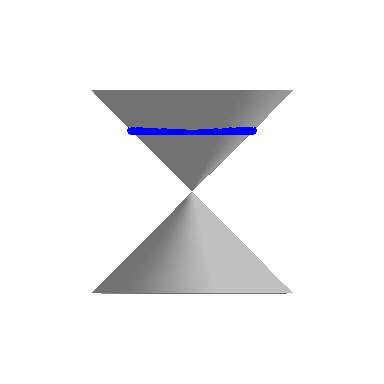
\includegraphics[width=2in]{./IntrotoConicsGraphics/Circle01.jpg} & 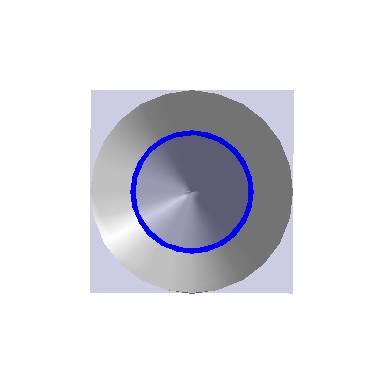
\includegraphics[width=2in]{./IntrotoConicsGraphics/Circle02.jpg} \\

\end{tabular}

\end{center}

\pagebreak

Tilting the plane ever so slightly produces an \index{ellipse ! from slicing a cone} \textbf{ellipse}.

\begin{center}

\begin{tabular}{cc}

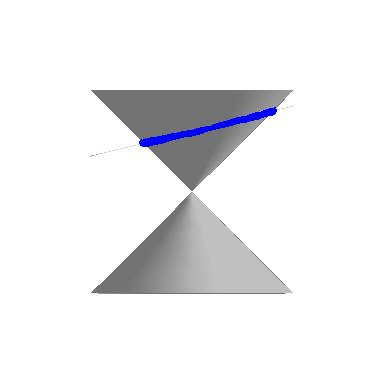
\includegraphics[width=2in]{./IntrotoConicsGraphics/Ellipse01.jpg} & 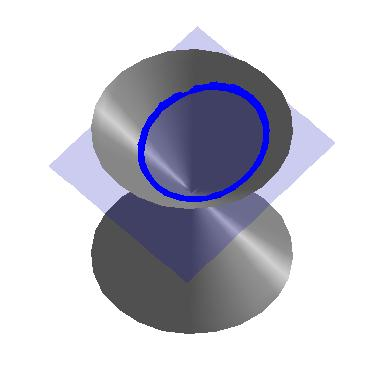
\includegraphics[width=2in]{./IntrotoConicsGraphics/Ellipse02.jpg} \\

\end{tabular}

\end{center}

If the plane cuts parallel to the cone, we get a \index{parabola ! from slicing a cone} \textbf{parabola}.

\begin{center}

\begin{tabular}{cc}

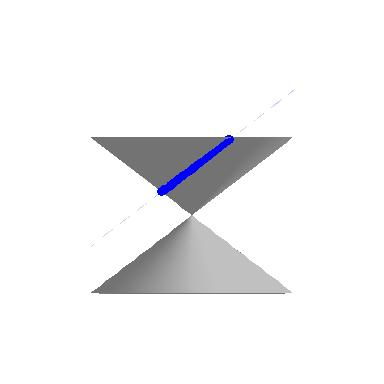
\includegraphics[width=2in]{./IntrotoConicsGraphics/Parabola01.jpg} & 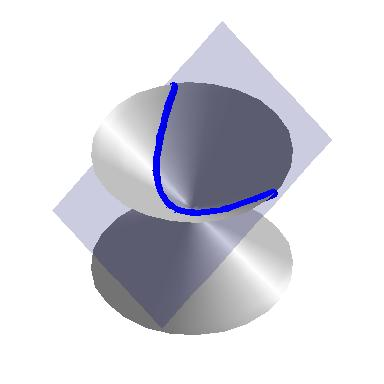
\includegraphics[width=2in]{./IntrotoConicsGraphics/Parabola02.jpg} \\

\end{tabular}

\end{center}

If we slice the cone with a vertical plane, we get a \index{hyperbola ! from slicing a cone} \textbf{hyperbola}.

\begin{center}

\begin{tabular}{cc}

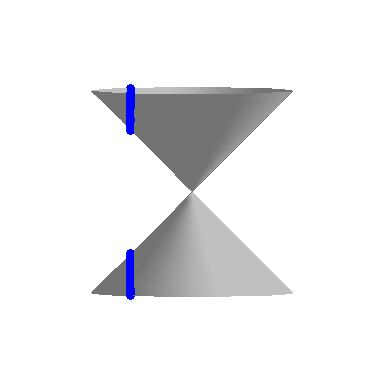
\includegraphics[width=2in]{./IntrotoConicsGraphics/Hyperbola01.jpg} & 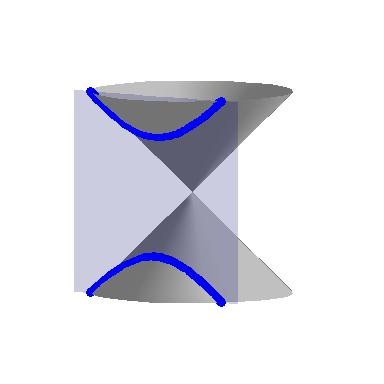
\includegraphics[width=2in]{./IntrotoConicsGraphics/Hyperbola02.jpg} \\

\end{tabular}

\end{center}


\pagebreak

If the slicing plane contains the vertex of the cone, we get the so-called `degenerate' conics:  a point, a line, or two intersecting lines.  

\phantomsection
\label{degenerateconics}

\begin{center}

\begin{tabular}{cc}

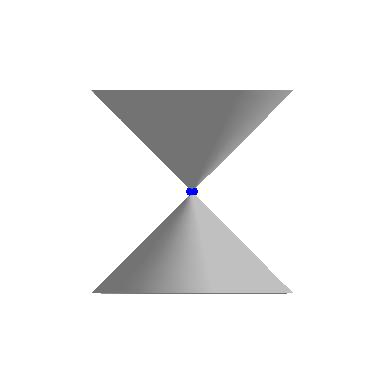
\includegraphics[width=2in]{./IntrotoConicsGraphics/Point01.jpg} & 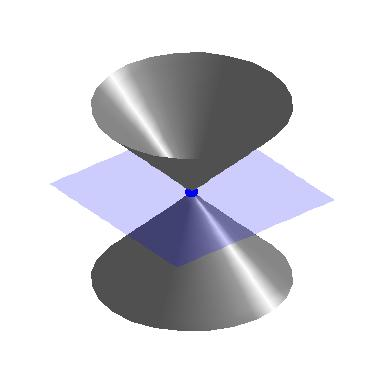
\includegraphics[width=2in]{./IntrotoConicsGraphics/Point02.jpg} \\


\includegraphics[width=2in]{./IntrotoConicsGraphics/Ilines01.jpg} & 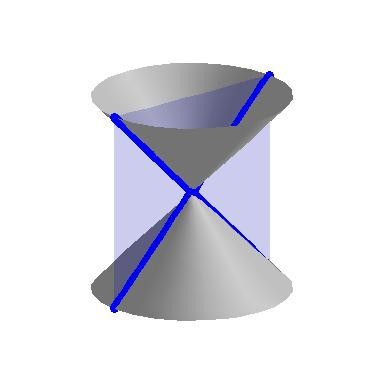
\includegraphics[width=2in]{./IntrotoConicsGraphics/Ilines02.jpg}\\

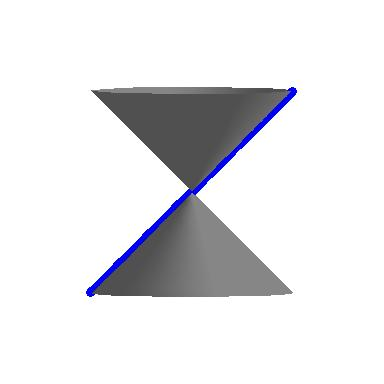
\includegraphics[width=2in]{./IntrotoConicsGraphics/Tline01.jpg} & 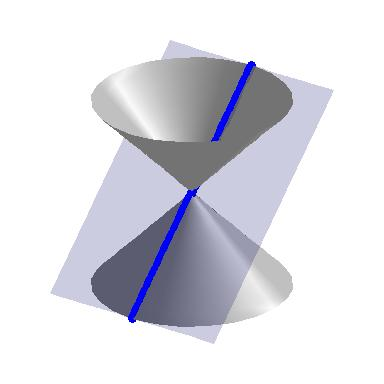
\includegraphics[width=2in]{./IntrotoConicsGraphics/Tline02.jpg} \\

\end{tabular}

\end{center}

\enlargethispage{.5in}
While this geometric introduction to the conic sections has its uses,\footnote{See Pierre Boulle's \textit{Planet of the Apes} for one example - we're serious!} in order to study the applications of the conic sections, we require a more analytic approach.  It turns out each of the  of the conic sections can be described as as a \textit{locus} of points - that is, a set of points which satisfy a certain condition involving distance.  The reader is referred to Section \ref{AppCartesianPlane} for a review of the distance and related formulas.

As we'll see, we'll be able to use the distance formula to algebraically represent the conic sections as  graphs of general quadratic equations in two variables.  That is, every conic section in the $xy$-plane can be represented as the graph of an equation of the form $Ax^2+Bxy+Cy^2+Dx+Ey +F = 0$ for real numbers $A$, $B$, $C$, $D$, $E$, and $F$.

\closegraphsfile